% ch8.tex
% This work is licensed under the Creative Commons Attribution-Noncommercial-Share Alike 3.0 New Zealand License.
% To view a copy of this license, visit http://creativecommons.org/licenses/by-nc-sa/3.0/nz
% or send a letter to Creative Commons, 171 Second Street, Suite 300, San Francisco, California, 94105, USA.


\chapter{Mais e mais tartarugas}\index{turtle!advanced}\label{ch:turtlesgalore}

Voltando ao módulo \code{turtle}, que começamos a ver no Capítulo~\ref{ch:turtles}. Lembre-se que para configurar a tela para a tartaruga desenhar, nós precisamos importar o módulo e criar um objeto `Pen':

\begin{listing}
\begin{verbatim}
>>> import turtle
>>> t = turtle.Pen()
\end{verbatim}
\end{listing}

Agora nós podemos usar algumas funções básicas para mover a tartaruga pela tela e desenhar algumas formas simples, mas seria interessante usar algo que nós já abordamos anteriormente. Por exemplo, o código que nós usamos para criar o quadrado, foi:

\begin{listing}
\begin{verbatim}
>>> t.forward(50)
>>> t.left(90)
>>> t.forward(50)
>>> t.left(90)
>>> t.forward(50)
>>> t.left(90)
\end{verbatim}
\end{listing} 

\noindent
Nós podemos reescrever esse código, usando um laço `for':

\begin{listing}
\begin{verbatim}
>>> t.reset()
>>> for x in range(1, 5):
...     t.forward(50)
...     t.left(90)
...
\end{verbatim}
\end{listing}

Que de fato é muito menos para se digitar, mas para algo ainda mais interessante, tente o seguinte:

\begin{listing}
\begin{verbatim}
>>> t.reset()
>>> for x in range(1, 9):
...     t.forward(100)
...     t.left(225)
...
\end{verbatim}
\end{listing}

Este código produz uma estrela de 8 pontas, como exibido na figura~\ref{fig20} (a tartaruga vira 225 graus, cada vez que anda 100 pixels para frente).

\begin{figure}
\begin{center}
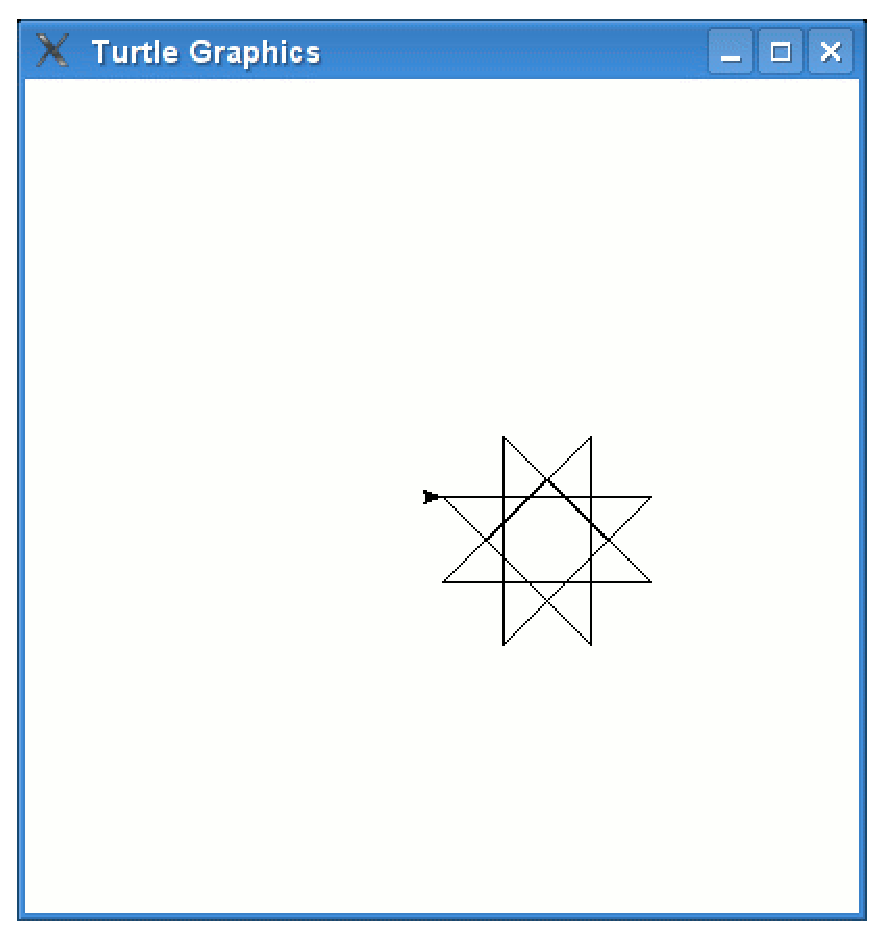
\includegraphics[width=72mm]{eps/figure20.eps}
\end{center}
\caption{A tartaruga desenhando uma estrela de 8 pontas.}\label{fig20}
\end{figure}

\noindent
Em um ângulo diferente (175 graus), e um laço mais longo (37 vezes), nós podemos fazer uma estrela com ainda mais pontas (como visto na figura~\ref{fig21}):

\begin{listing}
\begin{verbatim}
>>> t.reset()
>>> for x in range(1, 38):
...     t.forward(100)
...     t.left(175)
...
\end{verbatim}
\end{listing}

\begin{figure}
\begin{center}
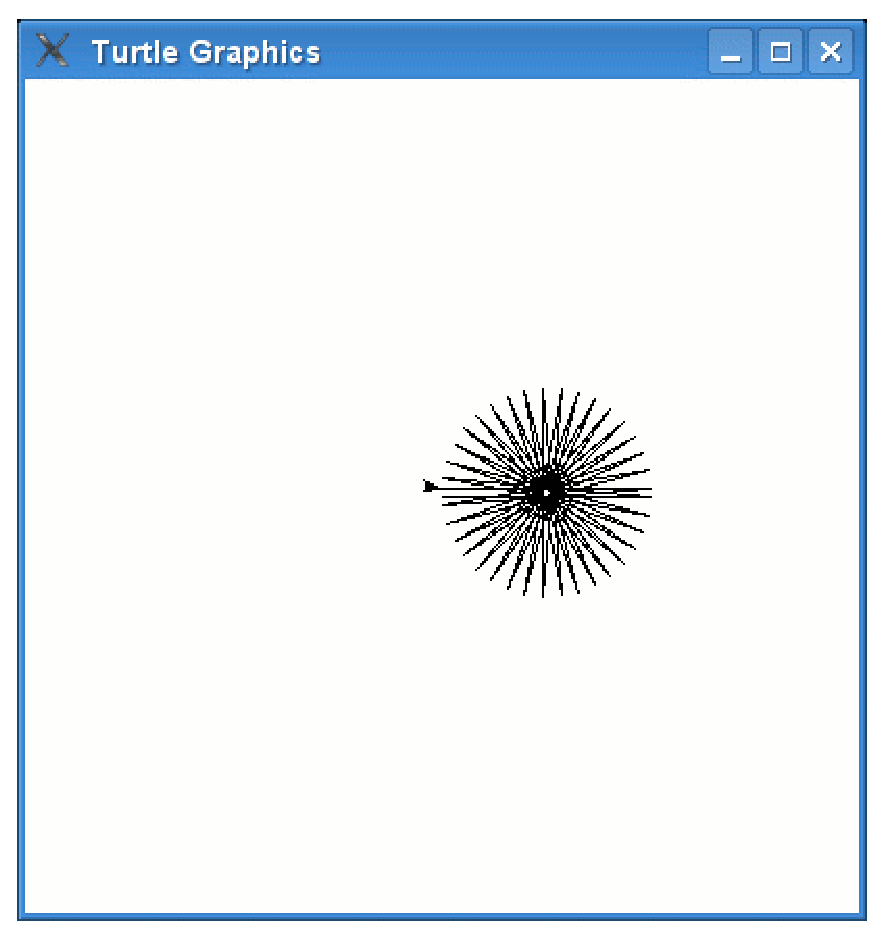
\includegraphics[width=72mm]{eps/figure21.eps}
\end{center}
\caption{Uma estrela com muito mais pontas.}\label{fig21}
\end{figure}

\noindent
Ou, que tal o seguinte código, que produz uma estrela tipo espiral, na figura~\ref{fig22}.

\begin{listing}
\begin{verbatim}
>>> for x in range(1, 20):
...     t.forward(100)
...     t.left(95)
...
\end{verbatim}
\end{listing}

\begin{figure}
\begin{center}
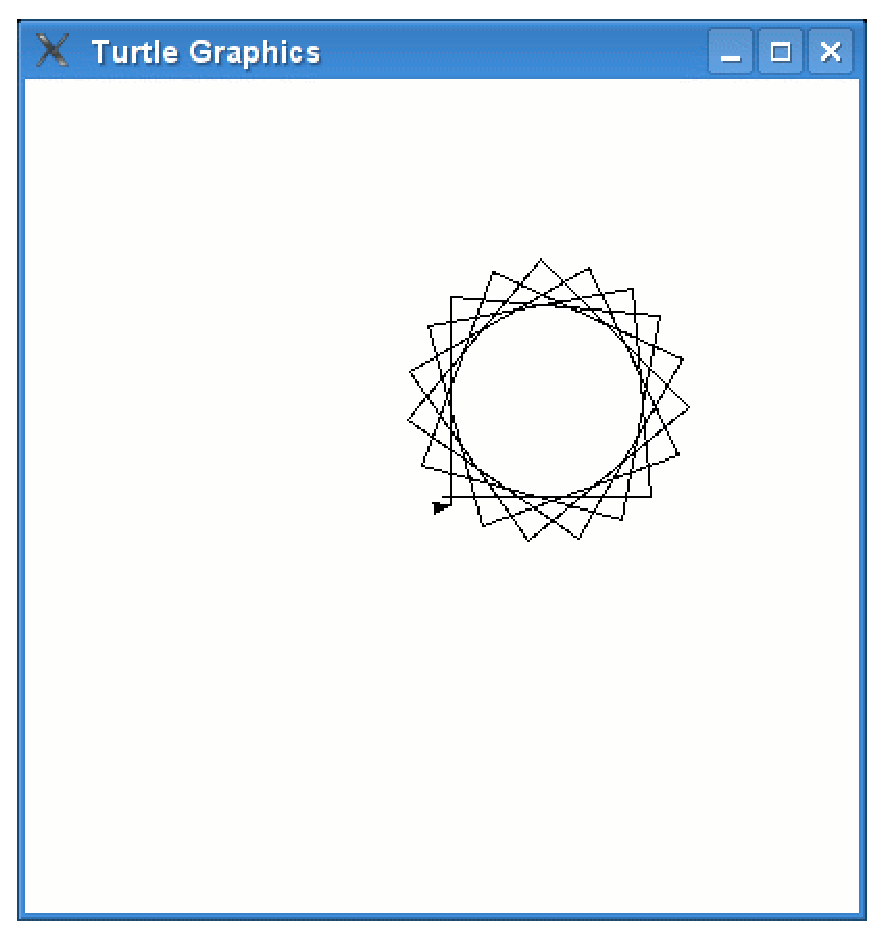
\includegraphics[width=72mm]{eps/figure22.eps}
\end{center}
\caption{Uma estrela tipo espiral.}\label{fig22}
\end{figure}

\noindent
Aqui está algo um pouco mais complicado:

\begin{listing}
\begin{verbatim}
>>> t.reset()
>>> for x in range(1, 19):
...     t.forward(100)
...     if x % 2 == 0:
...         t.left(175)
...     else:
...         t.left(225)
...
\end{verbatim}
\end{listing}

No código acima, nós verificamos se a variável \code{x} contém um número par. Para fazer isso, nós usamos um operador chamado módulo (\%)\index{modulo operator}, na expressão: \code{x \% 2 == 0}.
\par
x \% 2 é igual a zero, se o número na variável \code{x} puder ser dividido por dois, sem sobrar nada --- se isso não faz muito sentido, não se preocupe, apenas lembre de usar `\code{x \% 2 == 0}' para verificar se o número contido em uma variável é um número par. O resultado desse código, é uma estrela de 9 pontas, como na figura~\ref{fig23}.

\begin{figure}
\begin{center}
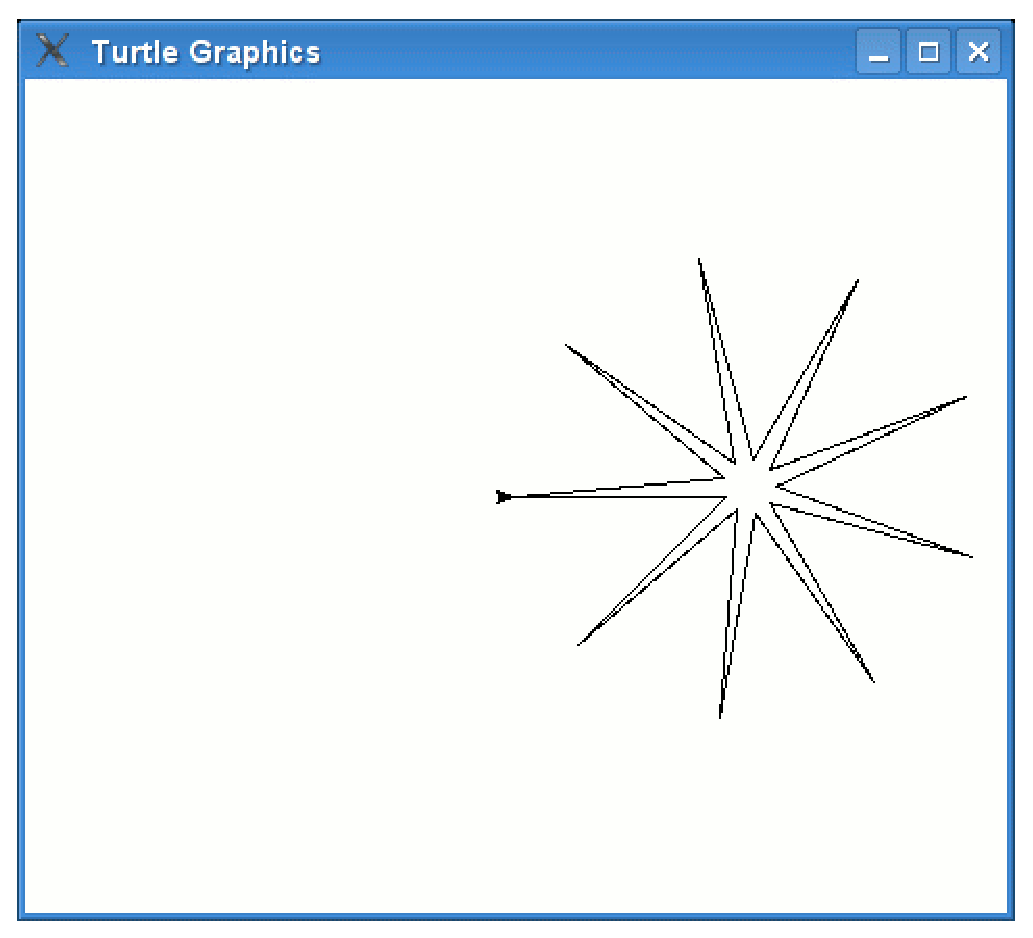
\includegraphics[width=84mm]{eps/figure23.eps}
\end{center}
\caption{Uma estrela de 9 pontas.}\label{fig23}
\end{figure}

Você não precisa apenas desenhar estrelas e simples formas geométricas. Usando uma combinação de chamadas de função, a sua tartaruga pode desenhar muitas coisas diferentes. Por exemplo:

\begin{listing}
\begin{verbatim}
t.color(1, 0, 0)
t.begin_fill()
t.forward(100)
t.left(90)
t.forward(20)
t.left(90)
t.forward(20)
t.right(90)
t.forward(20)
t.left(90)
t.forward(60)
t.left(90)
t.forward(20)
t.right(90)
t.forward(20)
t.left(90)
t.forward(20)
t.end_fill()
t.color(0, 0, 0)
t.up()
t.forward(10)
t.down()
t.begin_fill()
t.circle(10)
t.end_fill()
t.setheading(0)
t.up()
t.forward(90)
t.right(90)
t.forward(10)
t.setheading(0)
t.begin_fill()
t.down()
t.circle(10)
t.end_fill()
\end{verbatim}
\end{listing}

\noindent
Que é uma forma beeeem longa de se desenhar o carrinho feio e com visual bem primitivo, da figura~\ref{fig24}. Mas demonstra várias outras funções da tartaruga: \code{color}, para alterar a cor da caneta usada pela tartaruga, \code{fill}, que preenche uma área da tela; e \code{circle}, para desenhar um círculo com um determinado tamanho.

\begin{figure}
\begin{center}
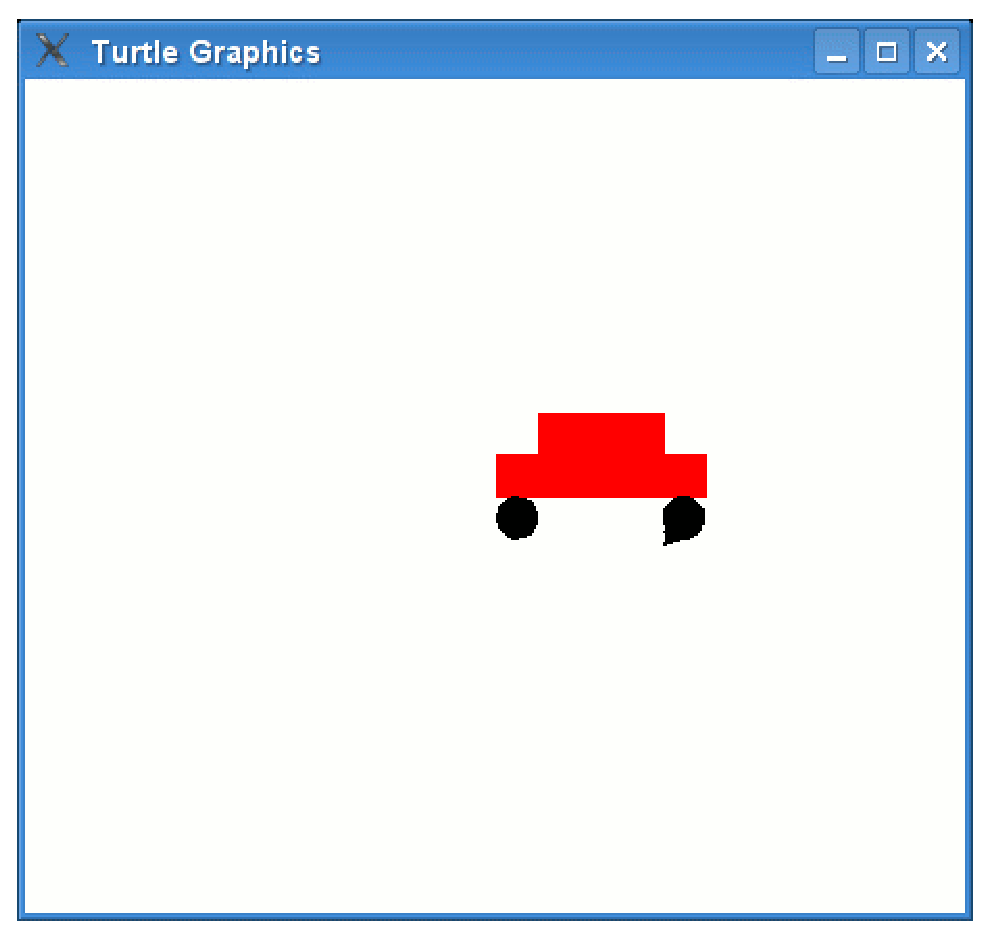
\includegraphics[width=80mm]{eps/figure24.eps}
\end{center}
\caption{A tartaruga é péssima em desenhar carros!}\label{fig24}
\end{figure}

\section{Colorindo}

A função \code{color}\index{turtle!color}, aceita 3 parâmetros. O primeiro parâmetro é o valor para o vermelho, o segundo é o valor para o verde e o último é o valor para o azul.
\par
\emph{Por que vermelho, verde e azul?}
\par
Se você já brincou com diferentes cores de tinta, você provavelmente já sabe parte da resposta para essa questão. Quando você mistura duas cores diferentes, você consegue outra cor\footnote{Na realidade, as três cores \textbf{primárias} são o vermelho, o amarelo e o azul e não vermelho/verde/azul (RGB -- Red/Green/Blue), no computador.}. Quando você mistura azul e vermelho, você consegue roxo$\ldots$ e quando você mistura várias cores, normalmente você consegue um marrom cor de lama. Em um computador, você pode misturar várias cores, da mesma forma --- coloca vermelho e verde juntos para conseguir amarelo --- exceto que com um computador, nós estamos combinando cores de luz, não cores de tinta.
 
Mesmo que não estejamos usando tinta, por um momento, pense em 3 potes grandes de tinta. Um vermelho, um verde e um azul. Os potes estão cheios, então nós vamos dizer que um pote cheio tem o valor de 1 (ou 100\%). Nós então derramamos todo o pote vermelho (100\%) em um tanque, seguido de toda a tinta verde (novamente, 100\%). Depois de misturar um pouco, nós teremos a cor amarela. Vamos desenhar um círculo amarelo usando a tartaruga:

\begin{listing}
\begin{verbatim}
>>> t.color(1, 1, 0)
>>> t.begin_fill()
>>> t.circle(50)
>>> t.end_fill()
\end{verbatim}
\end{listing}

Então acima, nós chamamos a função `color' com 100\% de vermelho (red), 100\% de verde (green) e 0\% de azul (blue) -- em outras palavras, 1, 1 e 0. Para facilitar o teste de outras cores, vamos transformar isso em uma função:

\begin{listing}
\begin{verbatim}
>>> def meucirculo(red, green, blue):
...     t.color(red, green, blue)
...     t.begin_fill()
...     t.circle(50)
...     t.end_fill()
...
\end{verbatim}
\end{listing}

\noindent
Nós podemos desenhar um círculo verde brilhante, usando toda a tinta verde (1 ou 100\%):

\begin{listing}
\begin{verbatim}
>>> mycircle(0, 1, 0)
\end{verbatim}
\end{listing}

\noindent
E nós podemos desenhar um círculo verde escuro, usando metade de toda a tinta verde (0.5 ou 50\%):

\begin{listing}
\begin{verbatim}
>>> meucirculo(0, 0.5, 0)
\end{verbatim}
\end{listing}

Aqui é onde pensar sobre tinta não faz muito sentido mais. No mundo real, se você tiver um pote de tinta verde, não importa o quanto você use, você sempre terá o mesmo tom. Com cores em um computador, devido a estarmos brincando com luzes, usando menos de uma cor geralmente resultará em uma tonalidade mais escura. É o mesmo que você acender uma tocha durante a noite, você terá uma luz amarelada --- quando a chama e a luz começarem a diminuir, a cor amarela começará a ficar mais e mais escura. Apenas para você ver, tente desenhar um círculo com um vermelho completo e um vermelho pela metade (1 e 0.5) e um azul completo e um azul pela metade.

\begin{listing}
\begin{verbatim}
>>> meucirculo(1, 0, 0)
>>> meucirculo(0.5, 0, 0)

>>> meucirculo(0, 0, 1)
>>> meucirculo(0, 0, 0.5)
\end{verbatim}
\end{listing}

\noindent
Diferentes combinações de vermelho, verde e azul produzirão uma enorme variedade de cores. Você terá a cor de ouro, usando 100\% do vermelho, 85\% do verde e nada do azul:

\begin{listing}
\begin{verbatim}
>>> meucirculo(1, 0.85, 0)
\end{verbatim}
\end{listing}

\noindent
Uma cor rosa claro pode ser feita combinando 100\% do vermelho, 70\% do verde e 75\% do azul:

\begin{listing}
\begin{verbatim}
>>> mycircle(1, 0.70,0.75)
\end{verbatim}
\end{listing}

\noindent
And you get orange by combining 100\% red and 65\% green; and brown by combining 60\% red, 30\% green and 15\% blue:

\begin{listing}
\begin{verbatim}
>>> mycircle(1, 0.65, 0)
>>> mycircle(0.6, 0.3, 0.15)
\end{verbatim}
\end{listing}

\noindent
Don't forget, you can clear the canvas by using \code{t.clear()}.

\section{Darkness}\index{turtle!color!black}

Here's a question for you:  What happens when you turn all the lights off at night? Everything goes black.
\par
The same thing happens with colours on a computer.  No light equals no colour.  So a circle with 0 for red, 0 for green and 0 for blue:

\begin{listing}
\begin{verbatim}
>>> mycircle(0, 0, 0)
\end{verbatim}
\end{listing}

Produces the black spot in figure~\ref{fig25}.

\begin{figure}
\begin{center}
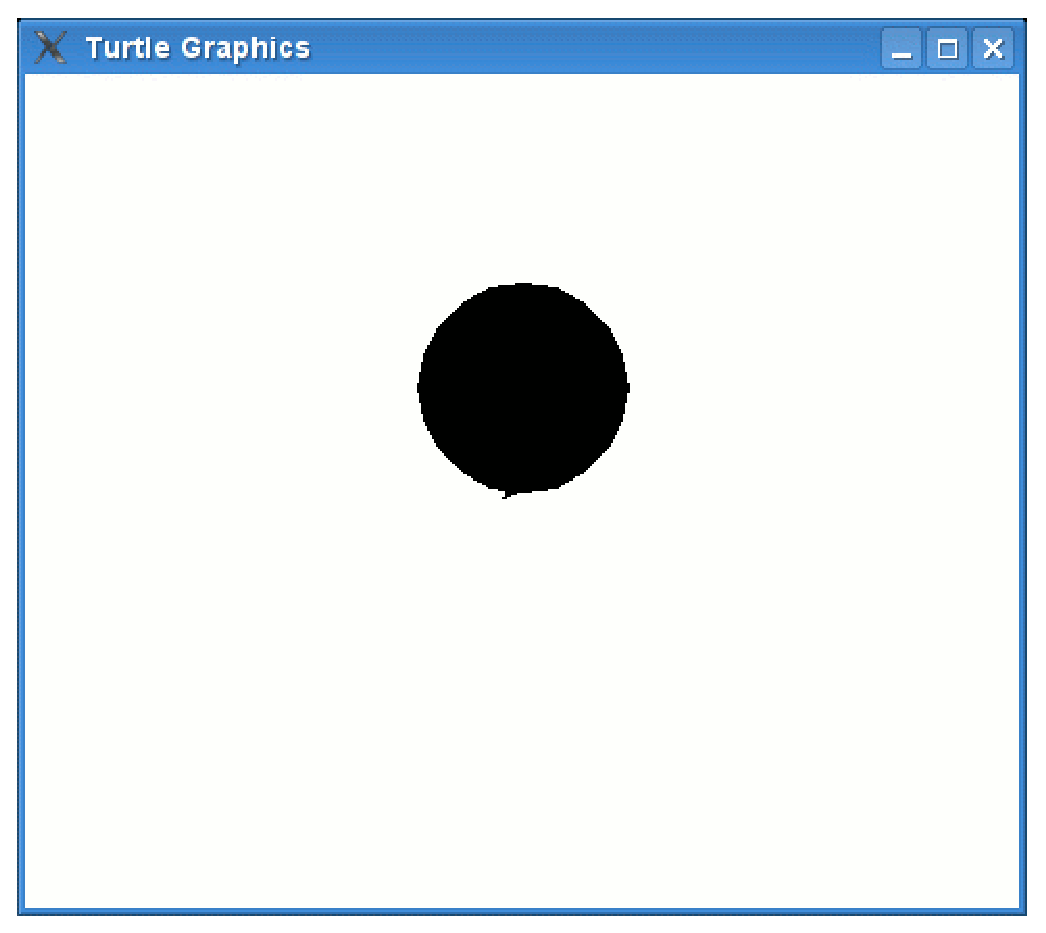
\includegraphics[width=85mm]{eps/figure25.eps}
\end{center}
\caption{A black hole!}\label{fig25}
\end{figure}

The opposite is true; if you use 100\% red, 100\% green and 100\% blue, you get white.  Use the following code and the black circle will be wiped out again:

\begin{listing}
\begin{verbatim}
>>> mycircle(1,1,1)
\end{verbatim}
\end{listing}

\section{Filling things}\index{turtle!fill}

You've probably figured out by now that the fill function is switched on by passing the parameter `1', then switched off again with `0'. When you switch it off, the function actually fills in the area you've drawn---assuming you've drawn at least part of a shape. So we can easily draw a filled in square by using code we created earlier. First, let's turn it into a function. To draw a square with turtle we do:

\begin{listing}
\begin{verbatim}
>>> t.forward(50)
>>> t.left(90)
>>> t.forward(50)
>>> t.left(90)
>>> t.forward(50)
>>> t.left(90)
>>> t.forward(50)
>>> t.left(90)
\end{verbatim}
\end{listing}

So as a function, we might want to pass the size of the square as a parameter.  This makes the function a little more flexible:

\begin{listing}
\begin{verbatim}
>>> def mysquare(size):
...     t.forward(size)
...     t.left(90)
...     t.forward(size)
...     t.left(90)
...     t.forward(size)
...     t.left(90)
...     t.forward(size)
...     t.left(90)
\end{verbatim}
\end{listing}

\noindent
We can test our function by calling:

\begin{listing}
\begin{verbatim}
>>> mysquare(50)
\end{verbatim}
\end{listing}

That's a start, but it's not quite perfect.  If you look at the code above, you'll see a pattern.  We repeat: \code{forward(size)} and \code{left(90)} four times.  That's a waste of typing.  So we can use a for-loop to do it for us (pretty much the same as we did earlier):

\begin{listing}
\begin{verbatim}
>>> def mysquare(size):
...     for x in range(0,4):
...         t.forward(size)
...         t.left(90)
\end{verbatim}
\end{listing}

That's a big improvement on the previous version. You can test the function with different sizes:

\begin{listing}
\begin{verbatim}
>>> t.reset()
>>> mysquare(25)
>>> mysquare(50)
>>> mysquare(75)
>>> mysquare(100)
>>> mysquare(125)
\end{verbatim}
\end{listing}

And the turtle should draw something like figure~\ref{fig26}.

\begin{figure}
\begin{center}
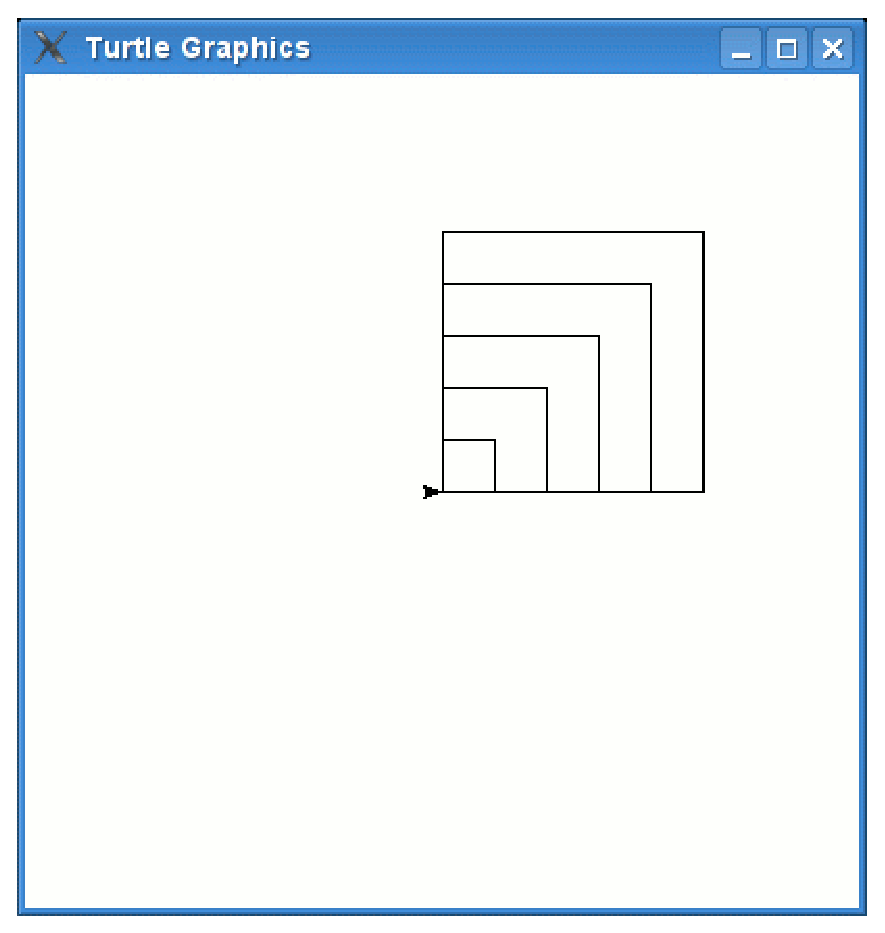
\includegraphics[width=72mm]{eps/figure26.eps}
\end{center}
\caption{Lots of squares.}\label{fig26}
\end{figure}

\noindent
Now we can try a filled square.  First of all, reset the canvas once again:

\begin{listing}
\begin{verbatim}
>>> t.reset()
\end{verbatim}
\end{listing}

\noindent
Then, turn on filling, and call the square function again:

\begin{listing}
\begin{verbatim}
>>> t.begin_fill()
>>> mysquare(50)
\end{verbatim}
\end{listing}

\noindent
You'll still see an empty square until you turn filling off:

\begin{listing}
\begin{verbatim}
>>> t.end_fill()
\end{verbatim}
\end{listing}

\noindent
Which produces something like the square in figure~\ref{fig27}.

\begin{figure}
\begin{center}
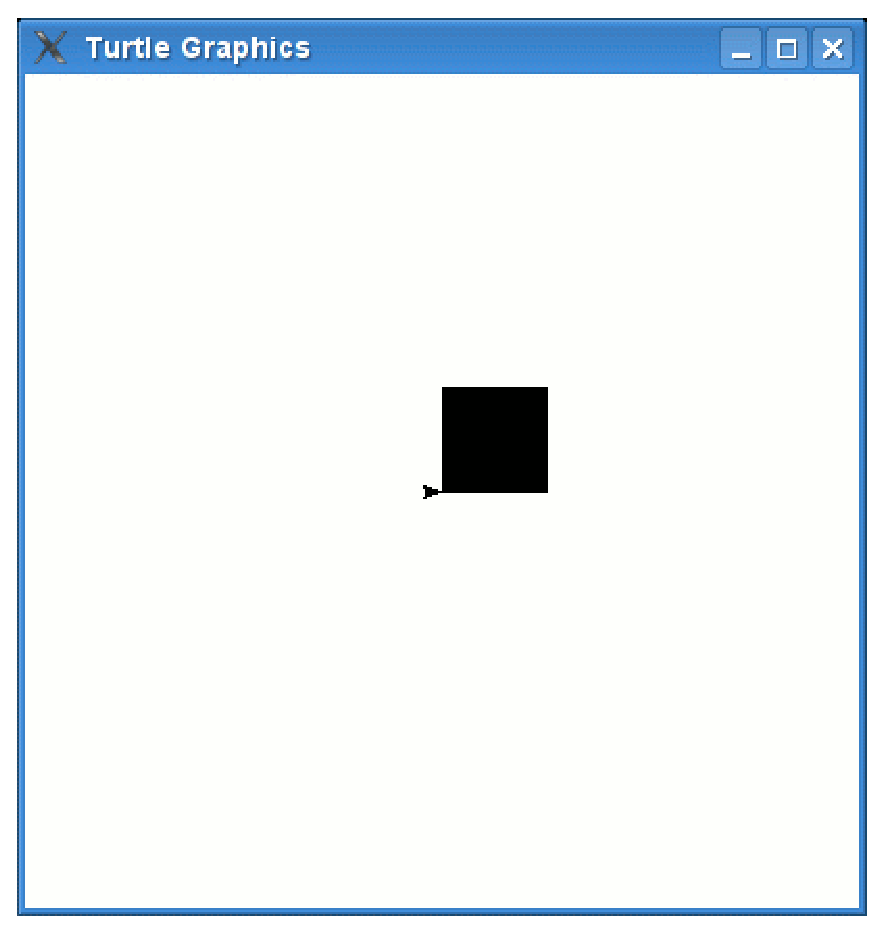
\includegraphics[width=72mm]{eps/figure27.eps}
\end{center}
\caption{A black square.}\label{fig27}
\end{figure}

How about changing the function so that we can either draw a filled or an unfilled square? We need another parameter, and slightly more complicated code, to do this:

\begin{listing}
\begin{verbatim}
>>> def mysquare(size, filled):
...    if filled == True:
...        t.begin_fill()
...    for x in range(0,4):
...        t.forward(size)
...        t.left(90)
...    if filled == True:
...        t.end_fill()
...
\end{verbatim}
\end{listing}

The first two lines check to see if the value of parameter `filled' is set to True. If it is, then filling is turned on.  We then loop four times to draw the four sides of the rectangle, before checking a second time whether the parameter `filled' is True, and if so, turn filling off once again. You can now draw a filled square by calling:

\begin{listing}
\begin{verbatim}
>>> mysquare(50, True)
\end{verbatim}
\end{listing}

\noindent
And an unfilled square by calling:

\begin{listing}
\begin{verbatim}
>>> mysquare(150, False)
\end{verbatim}
\end{listing}

\noindent
Which causes our turtle to draw the image in figure~\ref{fig28}$\ldots$ $\ldots$which, now that I think about it, looks like a weird square eye.

\begin{figure}
\begin{center}
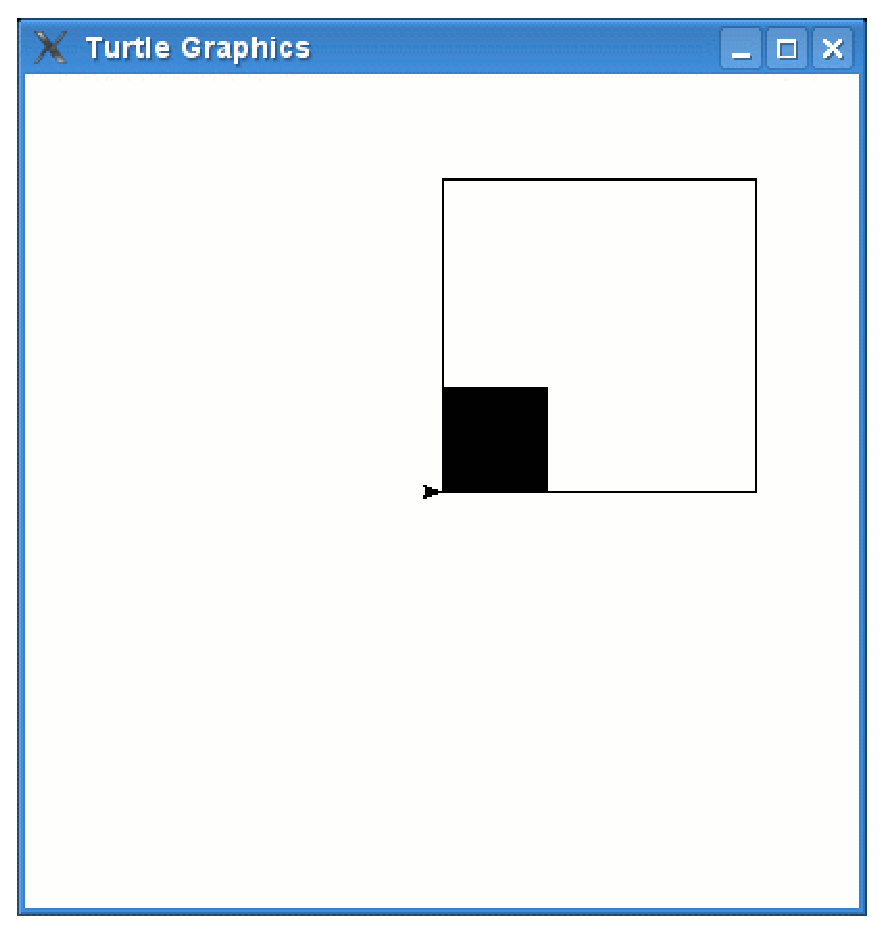
\includegraphics[width=72mm]{eps/figure28.eps}
\end{center}
\caption{A square eye.}\label{fig28}
\end{figure}

You can draw all sorts of shapes and fill them with colour. Let's turn the star, we drew earlier, into a function. The original code looked like this:

\begin{listing}
\begin{verbatim}
>>> for x in range(1,19):
...     t.forward(100)
...     if x % 2 == 0:
...         t.left(175)
...     else:
...         t.left(225)
...
\end{verbatim}
\end{listing}

We can use the same if-statements from the mysquare function, and use the size parameter in the \code{forward} function.

\begin{listing}
\begin{verbatim}
1.  >>> def mystar(size, filled):
2.  ...     if filled:
3.  ...         t.begin_fill()
4.  ...     for x in range(1,19):
5.  ...         t.forward(size)
6.  ...         if x % 2 == 0:
7.  ...             t.left(175)
8.  ...         else:
9.  ...             t.left(225)
10. ...     if filled:
11. ...         t.end_fill()
\end{verbatim}
\end{listing}

In lines 2 and 3, we switch filling on, depending upon the value of the parameter \code{filled} (turn filling on, if the parameter is set to True, turn it off, if the parameter is set to False).  We do the reverse in lines 10 and 11 (switch filling back off again).  The other difference about this function is that we pass the size of the star in the parameter \code{size}, and use this value in line 5.
\par
Now let's set the colour to gold (you might remember that gold can be made by using 100\% of red, 85\% of green and no blue), and then call the function:

\begin{listing}
\begin{verbatim}
>>> t.color(1, 0.85, 0)
>>> mystar(120, True)
\end{verbatim}
\end{listing}

\noindent
The turtle should draw the gold star in figure~\ref{fig29}. We can add an outline for the star, by changing the colour again (this time to black) and redrawing the star with filling turned off

\begin{figure}
\begin{center}
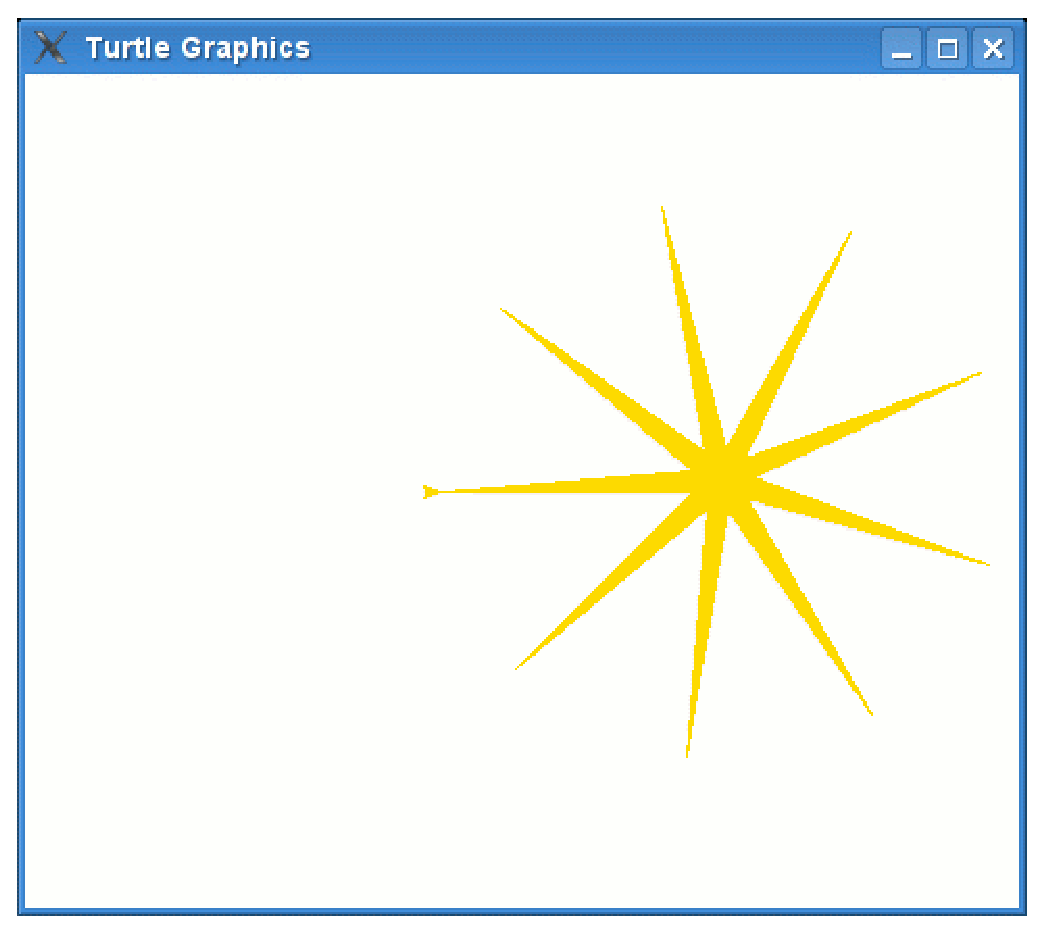
\includegraphics[width=85mm]{eps/figure29.eps}
\end{center}
\caption{A gold star.}\label{fig29}
\end{figure}

\begin{listing}
\begin{verbatim}
>>> t.color(0,0,0)
>>> mystar(120, False)
\end{verbatim}
\end{listing}

\noindent
Thus the star now looks like figure~\ref{fig30}.

\begin{figure}
\begin{center}
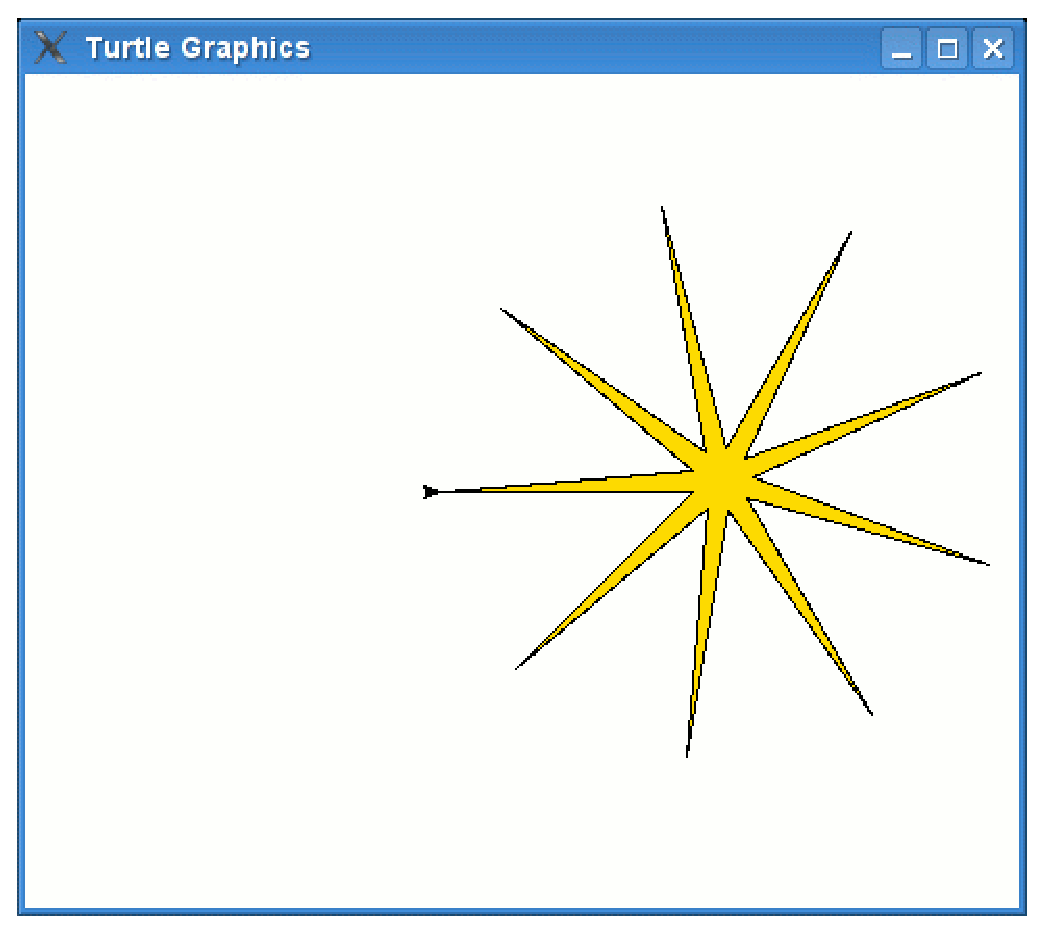
\includegraphics[width=85mm]{eps/figure30.eps}
\end{center}
\caption{A star with an outline.}\label{fig30}
\end{figure}

\section{Things to try}

\emph{In this chapter we learned about the turtle module, using it to draw a few basic geometric shapes. We used functions in order to re-use some of our code, to make it easier to draw shapes with different colours.}

\subsection*{Exercise 1}
We've drawn stars, squares and rectangles.  How about an octagon?  An octagon is an 8 sided shape.
(Hint: try turning 45 degrees).

\subsection*{Exercise 2}
Now convert the octagon drawing code into a function which will fill it with a colour.

\newpage
